\documentclass[]{article}\usepackage[]{graphicx}\usepackage[]{color}
%% maxwidth is the original width if it is less than linewidth
%% otherwise use linewidth (to make sure the graphics do not exceed the margin)
\makeatletter
\def\maxwidth{ %
  \ifdim\Gin@nat@width>\linewidth
    \linewidth
  \else
    \Gin@nat@width
  \fi
}
\makeatother

\definecolor{fgcolor}{rgb}{0.345, 0.345, 0.345}
\newcommand{\hlnum}[1]{\textcolor[rgb]{0.686,0.059,0.569}{#1}}%
\newcommand{\hlstr}[1]{\textcolor[rgb]{0.192,0.494,0.8}{#1}}%
\newcommand{\hlcom}[1]{\textcolor[rgb]{0.678,0.584,0.686}{\textit{#1}}}%
\newcommand{\hlopt}[1]{\textcolor[rgb]{0,0,0}{#1}}%
\newcommand{\hlstd}[1]{\textcolor[rgb]{0.345,0.345,0.345}{#1}}%
\newcommand{\hlkwa}[1]{\textcolor[rgb]{0.161,0.373,0.58}{\textbf{#1}}}%
\newcommand{\hlkwb}[1]{\textcolor[rgb]{0.69,0.353,0.396}{#1}}%
\newcommand{\hlkwc}[1]{\textcolor[rgb]{0.333,0.667,0.333}{#1}}%
\newcommand{\hlkwd}[1]{\textcolor[rgb]{0.737,0.353,0.396}{\textbf{#1}}}%
\let\hlipl\hlkwb

\usepackage{framed}
\makeatletter
\newenvironment{kframe}{%
 \def\at@end@of@kframe{}%
 \ifinner\ifhmode%
  \def\at@end@of@kframe{\end{minipage}}%
  \begin{minipage}{\columnwidth}%
 \fi\fi%
 \def\FrameCommand##1{\hskip\@totalleftmargin \hskip-\fboxsep
 \colorbox{shadecolor}{##1}\hskip-\fboxsep
     % There is no \\@totalrightmargin, so:
     \hskip-\linewidth \hskip-\@totalleftmargin \hskip\columnwidth}%
 \MakeFramed {\advance\hsize-\width
   \@totalleftmargin\z@ \linewidth\hsize
   \@setminipage}}%
 {\par\unskip\endMakeFramed%
 \at@end@of@kframe}
\makeatother

\definecolor{shadecolor}{rgb}{.97, .97, .97}
\definecolor{messagecolor}{rgb}{0, 0, 0}
\definecolor{warningcolor}{rgb}{1, 0, 1}
\definecolor{errorcolor}{rgb}{1, 0, 0}
\newenvironment{knitrout}{}{} % an empty environment to be redefined in TeX

\usepackage{alltt}
\usepackage{setspace}
\usepackage[margin = 1in]{geometry}
\usepackage[colorinlistoftodos]{todonotes}
\usepackage{amssymb,amsmath}
\usepackage{ifxetex,ifluatex}
\usepackage{fixltx2e} % provides \textsubscript
\ifnum 0\ifxetex 1\fi\ifluatex 1\fi=0 % if pdftex
  \usepackage[T1]{fontenc}
  \usepackage[utf8]{inputenc}
\else % if luatex or xelatex
  \ifxetex
    \usepackage{mathspec}
  \else
    \usepackage{fontspec}
  \fi
  \defaultfontfeatures{Ligatures=TeX,Scale=MatchLowercase}
\fi
% use upquote if available, for straight quotes in verbatim environments
\IfFileExists{upquote.sty}{\usepackage{upquote}}{}
% use microtype if available
\IfFileExists{microtype.sty}{%
\usepackage{microtype}
\UseMicrotypeSet[protrusion]{basicmath} % disable protrusion for tt fonts
}{}
\usepackage{hyperref}
\hypersetup{unicode=true,
            pdftitle={Chapter 1},
            pdfauthor={Frederick Boehm},
            pdfborder={0 0 0},
            breaklinks=true}
\urlstyle{same}  % don't use monospace font for urls
\usepackage{graphicx}
\makeatletter
\def\maxwidth{\ifdim\Gin@nat@width>\linewidth\linewidth\else\Gin@nat@width\fi}
\def\maxheight{\ifdim\Gin@nat@height>\textheight\textheight\else\Gin@nat@height\fi}
\makeatother
% Scale images if necessary, so that they will not overflow the page
% margins by default, and it is still possible to overwrite the defaults
% using explicit options in \includegraphics[width, height, ...]{}
\setkeys{Gin}{width=\maxwidth,height=\maxheight,keepaspectratio}
\IfFileExists{parskip.sty}{%
\usepackage{parskip}
}{% else
\setlength{\parindent}{0pt}
\setlength{\parskip}{6pt plus 2pt minus 1pt}
}
\setlength{\emergencystretch}{3em}  % prevent overfull lines
\providecommand{\tightlist}{%
  \setlength{\itemsep}{0pt}\setlength{\parskip}{0pt}}
\setcounter{secnumdepth}{0}
% Redefines (sub)paragraphs to behave more like sections
\ifx\paragraph\undefined\else
\let\oldparagraph\paragraph
\renewcommand{\paragraph}[1]{\oldparagraph{#1}\mbox{}}
\fi
\ifx\subparagraph\undefined\else
\let\oldsubparagraph\subparagraph
\renewcommand{\subparagraph}[1]{\oldsubparagraph{#1}\mbox{}}
\fi

%%% Use protect on footnotes to avoid problems with footnotes in titles
\let\rmarkdownfootnote\footnote%
\def\footnote{\protect\rmarkdownfootnote}

%%% Change title format to be more compact
\usepackage{titling}
\usepackage[
    backend=biber,
    style=authoryear,
    natbib=true,
    url=true, 
    doi=true,
    eprint=true,
    maxbibnames=10
]{biblatex}
\addbibresource{ch1.bib}
%\addbibresource{research.bib}
\addbibresource{../diss-latex/research.bib}

% Create subtitle command for use in maketitle
\newcommand{\subtitle}[1]{
  \posttitle{
    \begin{center}\large#1\end{center}
    }
}

\setlength{\droptitle}{-2em}

  \title{Chapter 1}
    \pretitle{\vspace{\droptitle}\centering\huge}
  \posttitle{\par}
    \author{Frederick Boehm}
    \preauthor{\centering\large\emph}
  \postauthor{\par}
      \predate{\centering\large\emph}
  \postdate{\par}
    \date{\today}
\IfFileExists{upquote.sty}{\usepackage{upquote}}{}
\begin{document}



\doublespacing
\maketitle

\listoftodos
\listoffigures
\listoftables

%lead up to need for MPP pleiotropy test. Discuss pleiotropy testing in 2-parent crosses
% as the second to last section


Quantitative trait locus (QTL) studies in model organisms like mice can identify 
genomic regions that affect quantitative traits, such as systolic blood pressure and body weight.
Tracing its origins back to \citet{sax1923association}, a genome-wide QTL ``scan'' discovers
associations between genotypes and phenotypes by considering every position, one at a time, as a candidate QTL for the trait of interest.
A region with strong evidence of association, then, defines a QTL. Because nearby markers have correlated
genotypes, a QTL in a two-parent cross often spans multiple megabases in length and may contain more than a hundred genes.
Identification of the causal gene from among those genes contained in the QTL is challenging and may require costly and time-consuming experiments. 
Growing needs for greater QTL mapping resolution fueled development, over the last two decades, of model organism multiparental populations for high-resolution QTL mapping.







% paragraph 2
Testing pleiotropy vs. separate QTL in model organisms can aid understanding of 
genetic architecture and reveal insights into biomolecular interactions in 
diverse areas including metagenomics, metabolomics, and behavioral genetics.
The need to test pleiotropy arises when two (or more) traits demonstrate evidence 
of univariate QTL in a single, shared genomic region. 



% funnel
Identifying a gene that affects multiple traits may inform scientific understanding of
interactions between biomolecules and ultimately contribute insights that aid development
of new therapeutics. 
%pleiotropy
For example, mouse studies identified multiple biological roles for products of 
the \emph{Agouti} gene. Mutations in the \emph{Agouti} gene may lead to both 
yellow hair (in mice that are typically black) and obesity \citep{attie2017how}.
Subsequent investigations uncovered two related biological roles for the Agouti protein.
It antagonizes the action of $\alpha$-melanocyte-stimulating hormone both to
prevent melanocyte-based melanin production and to disrupt melanocortin-4 receptor signaling in the brain.
The former leads to yellow hair, while the latter causes weight gain.
Later research identified altered signaling by the melanocortin-4 receptor in the brain as a leading cause of inherited obesity in humans.
Therapeutics to mitigate the effects of \emph{Agouti} mutations are currently being studied.


\begin{figure}
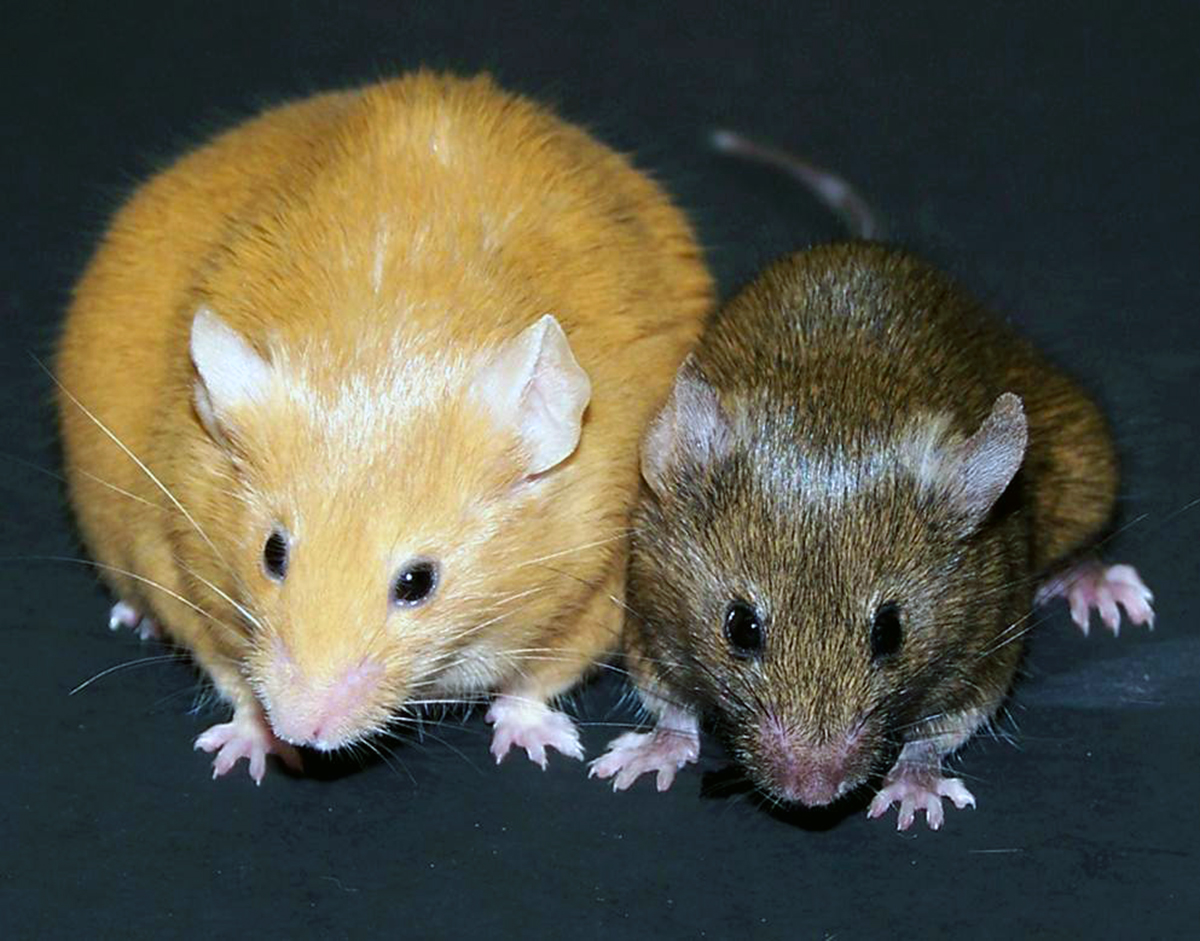
\includegraphics[height=6cm]{figs/Agouti.jpg}
\caption{\emph{Agouti} viable-yellow mutant mouse has yellow hair and is obese in comparison to a wild-type mouse. \tiny{(https://upload.wikimedia.org/wikipedia/commons/4/4d/Agouti\_Mice.jpg)}}
\label{fig:agouti}
\end{figure}


DNA variants that affect a trait like systolic blood pressure
can be identified by systematically looking for correlations with genotypes at different positions across the genome.

Complex traits include
clinical measurements, such as systolic blood pressure and body weight, as
well as newly measurable biomolecular traits like gene expression
levels, protein concentrations, and lipid levels.
Understanding the
genetics of complex traits may inform the fields of biology,
medicine, and public health.
%two-parent designs: intercross & backcross


%mapping populations
Multiparental populations of model organisms are designed with the goals of 
incorporating many genetic variants and enhancing QTL mapping resolution.
For much of the 20th century, researchers used two-parent crosses to identify large QTL that affect complex traits. 
Beginning in the late 1900s and early 2000s, geneticists recognized the limitations 
of two-parent QTL study designs. 
Due to the limited number of cumulative recombination events, existing two-parent study designs provided limited mapping resolution. 
Additionally, crosses of two inbred lines limits the collection of genetic variants in the offspring.
A study design that incorporates DNA from more than two inbred lines would capture a greater number of genetic variants. 
Since mapping resolution is related to the cumulative number of meiotic crossover 
events on a chromosome, it would also be advantageous to have multi-generational mapping
populations, in contrast to the traditional two-generation populations
that result from backcrosses and intercrosses in two-parent designs.


%mice






% genotype data & hmm to infer 36-state genotype probabilities

\begin{figure} % courtesy of Karl Broman & S. Sen (2009)
\setlength{\unitlength}{0.7cm}
\centering
\begin{picture}(15,4)

% dots
\put(0,1.0){\circle{0.3}}
\put(2.5,1.0){\circle{0.3}}
\put(5,1.0){\circle{0.3}}
\put(10,1.0){\circle{0.3}}
\put(15,1.0){\circle{0.3}}
\put(0,2.5){\circle{0.3}}
\put(2.5,2.5){\circle{0.3}}
\put(5,2.5){\circle{0.3}}
\put(10,2.5){\circle{0.3}}
\put(15,2.5){\circle{0.3}}

% vectors
\thicklines
\put(0,1.3){\vector(0,1){0.9}}
\put(2.5,1.3){\vector(0,1){0.9}}
\put(5,1.3){\vector(0,1){0.9}}
\put(10,1.3){\vector(0,1){0.9}}
\put(15,1.3){\vector(0,1){0.9}}

\put(0.6,1.0){\vector(1,0){1.3}}
\put(3.1,1.0){\vector(1,0){1.3}}
\put(5.6,1.0){\vector(1,0){1.3}}
\put(8.1,1.0){\vector(1,0){1.3}}
\put(10.6,1.0){\vector(1,0){1.3}}
\put(13.1,1.0){\vector(1,0){1.3}}

% the tiny dots
\put(7.2,1.0){\circle*{0.05}}
\put(7.5,1.0){\circle*{0.05}}
\put(7.8,1.0){\circle*{0.05}}
\put(12.2,1.0){\circle*{0.05}}
\put(12.5,1.0){\circle*{0.05}}
\put(12.8,1.0){\circle*{0.05}}

% symbols
\put(-0.2,0){$G_1$}
\put(2.3,0){$G_2$}
\put(4.8,0){$G_3$}
\put(9.75,0){$G_i$}
\put(14.75,0){$G_n$}

\put(-0.2,3.0){$O_1$}
\put(2.3,3.0){$O_2$}
\put(4.7,3.0){$O_3$}
\put(9.75,3.0){$O_i$}
\put(14.75,3.0){$O_n$}
\end{picture}
\caption{Illustration of a hidden Markov model. $G$'s indicate
  underlying genotypes; $O$'s indicate observed marker
  phenotypes.\label{figD:hmm}} 
\end{figure}





%mapping genetic markers to measurable traits






%complex traits











%my test





%roadmap
Below, I present background material on statistical methods in quantitative trait locus
(QTL) mapping.
AfterI begin with an overview of
QTL mapping in two-parent crosses.
I then discuss pleiotropy testing in two-parent crosses before considering newly
developed multiparental populations.
I present the design for one multiparental population, the Diversity Outbred mice.
I close the first chapter by arguing for the need for a pleiotropy test for multiparental populations.


\subsection{Two-parent crosses}

\begin{knitrout}
\definecolor{shadecolor}{rgb}{0.969, 0.969, 0.969}\color{fgcolor}\begin{figure}
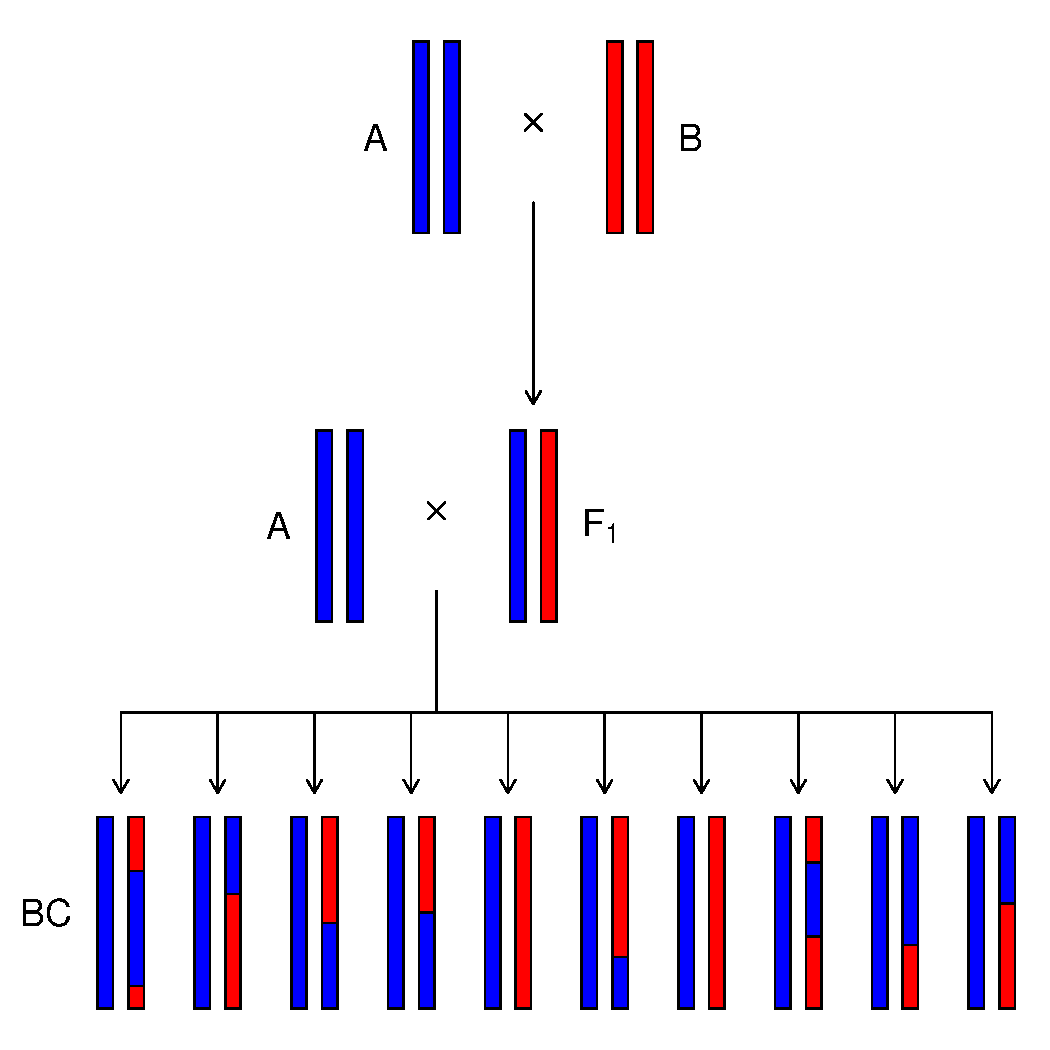
\includegraphics[width=\maxwidth]{figure/backcross-1} \caption[Breeding scheme for a backcross]{Breeding scheme for a backcross. Each pair of autosomes represents a single subject.}\label{fig:backcross}
\end{figure}


\end{knitrout}





\subsection{QTL mapping in two-parent crosses}

QTL mapping is a systematic, statistical approach to identifying genetic
loci where genetic variation affects phenotypic variation in a measured trait.
We use the term ``locus'' to refer to a small, contiguous genomic region, often
several megabases in length. Standard inputs are genome-wide marker genotypes for a collection of study subjects and a set of trait measurements on the same subjects.

% QTL scan (univariate)
A univariate QTL scan is a procedure to interrogate the entire genome for genetic
variants that affect a specified trait of interest.
It requires as inputs genome-wide marker genotypes (or, equivalently,
genotype probabilities) and trait measurements for a collection of subjects.
One specifies a statistical model and calculates the
likelihood of the model parameters given the observed (trait and marker) data at every marker. In studies with dense marker sets, 
it may suffice to calculate likelihoods only at the markers. However, for
studies with fewer markers, investigators often benefit from inferring 
genotype probabilities at inter-marker positions.


After obtaining likelihoods for all markers, likelihood ratio test statistics are calculated
at every marker. The inputs for these calculations are the likelihoods from the model fits at
every marker and the likelihood for the null model, which contains no genotype data.
The resulting likelihood ratios compare, for every marker, the null hypothesis that there is no 
QTL (at that marker) against the alternative that there is a QTL (at the specified marker).
In other words, one performs a likelihood ratio test for every marker across the genome.
Often this amounts to thousands of (statistically dependent) hypothesis tests.
One then uses a permutation test to determine a genome-wide critical value
for the likelihood ratio test statistic \citep{churchill1994empirical}.
Those loci for which the likelihood ratio test statistic is sufficiently large are declared QTL. 

Modern QTL studies have their origins in the work of \citet{sax1923association}.
\citet{sax1923association}, working 30 years before \citet{watson1953molecular} reported
the molecular structure of DNA, studied seed color and weight in the common bean
(\emph{Phaseolus vulgaris}). He used seed color to partition beans into genetic
marker classes and identified an association between marker class and bean weight. Implicitly, \citet{sax1923association} leveraged the association between marker genotype class and seed color to assign beans to genetic marker classes without having explicit genotype data.



\citet{lander1989mapping}, in a landmark methodology report, presented
interval mapping as a strategy to identify QTL. 
In interval mapping, they used the correlations between genetic markers
to infer genotype probabilities between markers.
They then use an expectation maximization algorithm \citep{dempster1977maximum, lander1987construction}
to fit a statistical mixture model with a normally distributed component for each of three genotype classes. 
They summarized the evidence for a QTL at each position with the log odds (LOD) score statistic.
The LOD score is the base 10 log likelihood ratio test statistic for
the competing hypotheses of the presence of a QTL at the candidate position
against the null hypothesis of no QTL at the candidate position. 
The work of \citet{lander1989mapping} fueled interest in QTL mapping from
both biologists and statisticians.
Many of the open questions that \citet{lander1989mapping} present, including approaches
for defining QTL endpoints, accounting for multiple hypothesis tests, and
allowing for genotyping errors when inferring genotype probabilities,
are active areas of research 30 years after their publication.








%statistical challenges in QTL mapping
Two major statistical challenges are what \citet{broman2009guide} call 
the ``missing data'' problem and the ``model selection'' problem. 
The ``missing data'' problem arises in QTL studies because genotypes are obtained
at only select markers. In this sense, genotypes at positions between
markers are ``missing'' because they aren't explicitly measured.
A flexible framework for resolving the ``missing data'' problem involves a
hidden Markov model \citep{broman2009guide, broman2006use}. 
In this hidden Markov model, marker genotypes are observed random variables, 
while genotypes at intervening bases are unobserved random variables \citep{broman2009guide,broman2006use}. 
Two sets of recursive equations, termed ``forward'' and ``backward'' equations,
enable efficient calculation of genotype probabilities
(conditional on the observed marker genotypes) \citep{baum1970maximization}.


%

% relationship between peak position and QTL 2-lod interval - NO




% model form - linear regression
A QTL analysis involves choosing a statistical model to be fitted at every marker. 
As in any statistical modeling, there is not one best model selection procedure.
One needs to decide which main effects and interactions are needed.
Also, one often transforms the trait values to achieve approximate normality before performing the QTL scan. 

Many investigators consider multiple models before performing a QTL scan.
For simplicity, one may choose a linear model that contains additive effects for
the  minor allele count (0, 1 or 2) at a given marker (Equation~\ref{eq:uni-2-parent}) \citep{martinez1992estimating,haley1992simple}.

\begin{equation}
\text{trait} = \text{mean for major allele homozygotes} + \text{(minor allele count)}\text{(minor allele effect)} + \text{random error}
\label{eq:uni-2-parent}
\end{equation}

Assuming that the random errors are normally distributed (and independent with common
variance $\sigma^2$), one may use the statistical technique called ``ordinary least squares''
to fit the model and to solve for $\hat b$ and $\hat \sigma^2$.
In ``ordinary least squares'', one solves for the set of parameter values that
minimize the residual sum of squares. In the above equation, our two parameters are the minor allele effect and the random error variance. The residual sum of squares is an expression that tells us how far each observed data point is from its predicted value for a set of specified parameter values. Equation~\ref{} defines residual sum of squares for a univariate QTL analysis.

\begin{equation}
\text{residual sum of squares} = \left(\text{fitted trait value} - \text{observed trait value}\right)^2
\end{equation}













% QTL scan (multivariate) in 2-parent crosses

In anticipation that multivariate mapping of correlated traits would enhance statistical power to detect QTL and would improve precision of QTL positions, both \citet{jiang1995multiple} and \citet{korol1995interval} developed multivariate interval mapping procedures. \todo[inline]{say more here}

In the context of multivariate QTL mapping, \citet{jiang1995multiple} 
proposed and developed a statistical hypothesis test for distinguishing
a single pleiotropic locus that affects multiple traits from two (or more)
separate QTL.
Their test applies to the setting in which multiple traits
map to a single genomic region \citep{jiang1995multiple}. 
That region, then, can be interrogated further by asking whether it
harbors a single pleiotropic QTL or multiple separate QTL. For simplicity, we focus on the case where two traits both map to a single genomic region, and we wish to determine whether the two traits share a single QTL or have two separate QTL. 











\subsection{Multiparental populations and Diversity Outbred mice}

Near the turn of the century, geneticists sought a mammalian gene mapping resource 
that could be used for study of a wide variety of quantitative traits. 
The magnitude of such an undertaking required a collaborative, community-supported approach \citep{de2014genetics}. Scientists conceived of the Diversity Outbred (DO) mouse population as such a high-resolution gene mapping resource. They elected to seed the population with partially inbred progenitors of the Collaborative Cross mouse population. The Collaborative Cross mating design started with mice from eight inbred lines: A/J, C57BL/6J, 129S1/SvImJ, NOD/ShiLtJ, NZO/HILtJ, CAST/EiJ, PWK/PhJ, WSB/EiJ.

The designers of the Collaborative Cross used a ``multi-funnel'' mating scheme to generate mice with DNA from all eight founder lines over the course of 3 generations. For example, in one funnel, mating pairs are: A x B, C x D, E x F, and G x H in the first generation. AB offspring would then mate with CD offspring and EF offspring would mate with GH mice. Finally, the ABCD mice would mate with the EFGH mice to create a generation of mice that contain genetic material from all eight inbred founder lines. Subsequent generations of inbreeding resulted in multiple inbred lines for the Collaborative Cross. \todo[inline]{make this figure}

The designers of the Diversity Outbred population started with \todo[inline]{get number of mice and from which generations}

Due to the breeding scheme, each Diversity Outbred mouse is a highly heterozygous mosaic of 
founders' DNA (Figure)\todo{add figure with mosaics over multiple generations here}. 
With each generation, the Diversity Outbred mice accumulate meiotic recombinations. 
This is because each mouse inherits DNA from its parents, and each meiosis provides opportunities for recombinations. \todo[inline]{need to explain this better. How does Andrew explain it in his thesis?}

The cumulative effect of recombinations over many generations of outbreeding is to create mice whose DNA mosaic contains smaller and smaller contiguous pieces from each founder line. 

The Diversity Outbred mice enable high-resolution QTL mapping \citep{gatti2014quantitative}. One factor that contributes to high-resolution mapping is the ability to infer the founder line from which each marker's DNA arose. 




\subsection{QTL mapping in DO mice}

QTL mapping in Diversity Outbred mice, like that in mice from two-parent crosses, is a multi-step procedure: 1. data acquisition, 2. inference of missing genotypes, and 3. modeling phenotypes as a function of genotypes. Data acquisition involves measurement of phenotypes and, at specified genetic markers, termed ``single nucleotide polymorphism'' or SNP markers, measurement of two-allele genotypes. Often, the SNP marker genotypes are obtained by use of a microarray, such as the GigaMUGA SNP microarray \citep{morgan2015mouse}. 

The next step, missing genotypes inference, is needed because of the ``missing data problem'' \citep{broman2009guide}. It takes as input the two-allele genotypes at the measured SNP markers. An expectation maximization algorithm \citep{dempster1977maximum} for a hidden Markov model, developed by \citet{broman2012haplotype} and \citet{broman2012genotype} and implemented in the \texttt{qtl2} R package \citep{broman2019rqtl2}, outputs 36-state genotype probabilities for all nuclear autosomal markers and pseudomarkers. Pseudomarkers, as we use the term, are arbitrary nucleotide bases at which the researcher wants 36-state genotype probabilities. Finally, we collapse the 36-state genotype probabilities to eight founder allele dosages at each marker. This last step is optional, but often helpful, because the simplified models require specification of fewer parameters. We then treat the founder allele dosages as known quantities in subsequent steps. 

% model form - connecting genotype to phenotype

After inferring founder allele dosages, we address the second major statistical challenge of 
QTL mapping: the ``model selection'' problem \citep{broman2009guide}.
Linear regression is widely used because of its ease of implementation,
computational speed, and interpretability of results.
A genetically ``additive'' linear model, in which we assume a linear relationship between
a trait and each founder allele's dosage, is widely used 
\citep{gatti2014quantitative,broman2019rqtl2}.
The R package \texttt{qtl2} provides a straightforward user
interface to include covariates and interaction terms in the linear model \citep{broman2019rqtl2}.




% model form - random effects incorporation & relatedness





\subsection{Testing pleiotropy in two-parent crosses}

\citet{jiang1995multiple} developed a suite of methods for analyzing multivariate phenotypes in
two-parent crosses.
Among the novel methods in their article is a test of pleiotropy vs separate QTL.
They explain that such a test is useful when two traits map to a single genomic region.
The question then arises ``do the two traits associate with the same locus, or do they associate with separate loci''?

If both traits associate with the same locus, then that locus is called ``pleiotropic''. If the two traits associate with separate loci, then we say that there are separate QTL (one for each trait). While ``pleiotropy'' has multiple related usages in the genetics literature, we use ``pleiotropy'' here to refer to the situation in which one genetic locus affects two or more traits. 

In the development of their test of pleiotropy v separate QTL, \citet{jiang1995multiple} model
the multivariate phenotype as the sum of a linear function of the genotypes and a random error term. They assume that the phenotypes matrix is related to the genotypes data (for a single marker) through the following equation:


\begin{equation}
Y = XB + E
\end{equation}


\noindent Where Y is a n by 2 matrix of phenotype values (with each row being one subject and each column being one trait)
, X is a n by 1 matrix of genotypes and B is a 1 by 2 matrix of allele effects.
The random error is assumed to follow a normal distribution with mean zero and a positive variance.
\citet{jiang1995multiple} also incorporate additional terms to model dominant effects and to
control for residual genetic variation.
We forego inclusion of dominant terms and additional markers for controlling residual
genetic variation, although, in our linear mixed effects model, we do include polygenic random
effects. 
Extensions of our model and software to accommodate dominance effects are straightforward.


\citet{jiang1995multiple} use a mixture model to relate genotypes to phenotypes. 
They observe that the there are 9 possible ordered pairs of genotypes for two markers in a F2 population, since each marker has one of three genotypes (AA, AB, BB).
They thus approach the problem as one with a 9-state mixture model. 
They provide the equations needed for an expectation-conditional maximization
(ECM) algorithm for fitting the mixture model.
They use a chi-square distribution with one degree of freedom as the
null distribution of the test statistic. 

Further investigations by \citet{jiang1995multiple} with simulations revealed
reasonable behavior of the hypothesis test under the specified conditions. 
They learned that dense marker coverage tends to aid in distinguishing pleiotropy
from separate QTL. \todo[inline]{IS THIS TRUE?? look back at JZ 1995's simulations. How did they examine power and type I error rates? Do they examine univariate LOD strength when considering power? What about interlocus distance?}










They use a computational algorithm called ``expectation - conditional maximization'' to find these values. 
ECM is an iterative algorithm. 
The user inputs starting values for the parameters and the algorithm changes them one at a
time until the change in log likelihood between successive iterations is sufficiently small.
The algorithm is then said to have ``converged''. 
The final iteration’s parameter values are treated as those that maximize the likelihood.


\citet{jiang1995multiple}, in the context of their multivariate QTL mapping methods, 
describe a test of pleiotropy vs. separate QTL. 
They formulate a test in which the null hypothesis
is pleiotropy while the the alternative hypothesis is separate QTL.
In other words, they consider the case in which the two traits map to the same locus
(pleiotropy) as a special case of the more general setting (separate QTL)
in which the two traits may or may not map to the same locus.

In statistical terminology, one would say that the parameter space is restricted under the null hypothesis. Here, the parameter space is the collection of ordered pairs of markers in the genomic region of interest. The restriction of that collection under pleiotropy corresponds to limiting consideration to only those ordered pairs that have both traits mapping to a single locus. 

\begin{knitrout}
\definecolor{shadecolor}{rgb}{0.969, 0.969, 0.969}\color{fgcolor}\begin{kframe}


{\ttfamily\noindent\itshape\color{messagecolor}{\#\# -- Attaching packages ------------------------------------------ tidyverse 1.2.1 --}}

{\ttfamily\noindent\itshape\color{messagecolor}{\#\# v ggplot2 3.1.0\ \ \ \ \ \  v purrr\ \  0.3.1\ \ \\\#\# v tibble\ \ 2.0.1\ \ \ \ \ \  v dplyr\ \  0.8.0.1\\\#\# v tidyr\ \  0.8.3\ \ \ \ \ \  v stringr 1.4.0\ \ \\\#\# v readr\ \  1.3.1\ \ \ \ \ \  v forcats 0.4.0}}

{\ttfamily\noindent\itshape\color{messagecolor}{\#\# -- Conflicts --------------------------------------------- tidyverse\_conflicts() --\\\#\# x .GlobalEnv::cross() masks purrr::cross()\\\#\# x dplyr::filter()\ \ \ \  masks stats::filter()\\\#\# x dplyr::lag()\ \ \ \ \ \ \ \ masks stats::lag()}}\end{kframe}
\end{knitrout}

\begin{knitrout}
\definecolor{shadecolor}{rgb}{0.969, 0.969, 0.969}\color{fgcolor}\begin{figure}
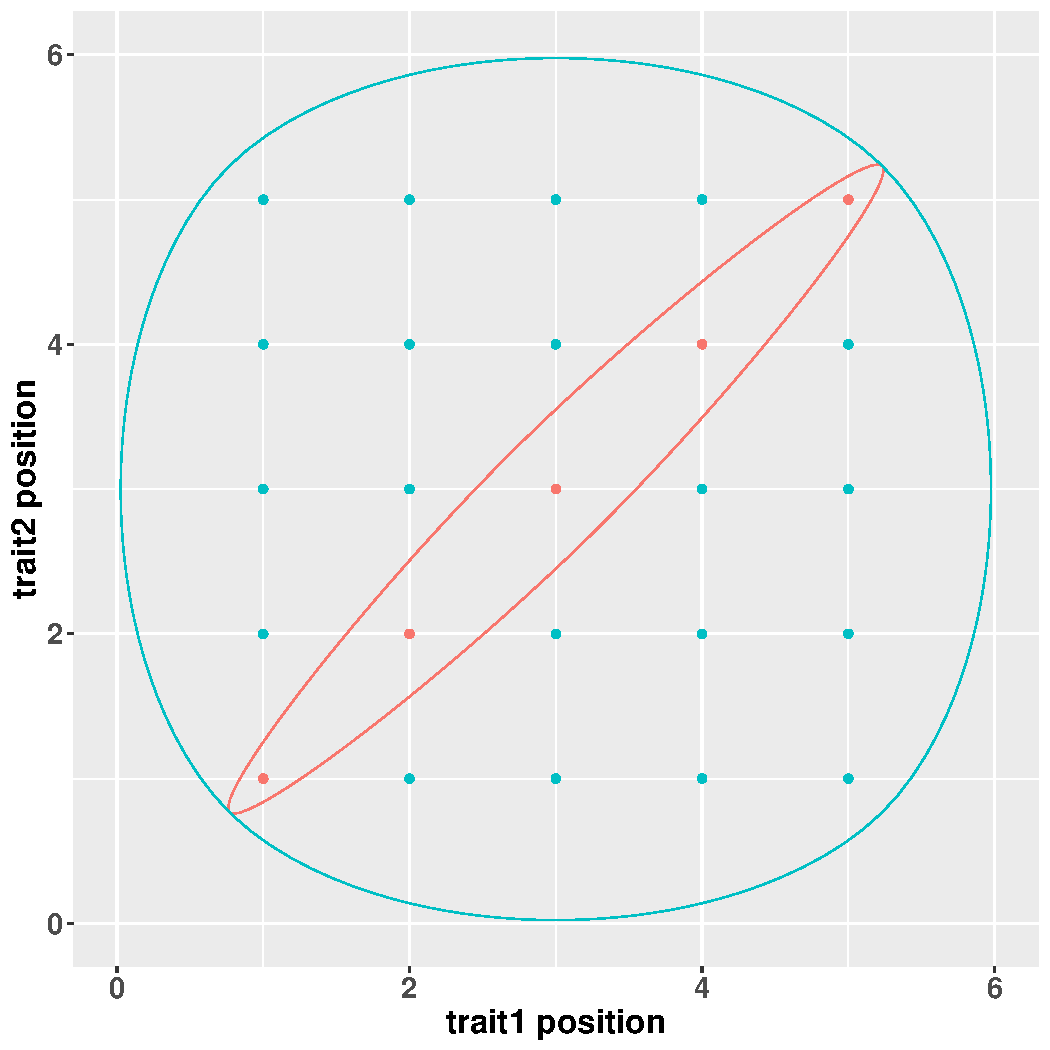
\includegraphics[width=\maxwidth]{figure/encircle-1} \caption[Two-dimensional grid of ordered pairs of markers]{Two-dimensional grid of ordered pairs of markers.}\label{fig:encircle}
\end{figure}


\end{knitrout}



\citet{jiang1995multiple} then calculate the likelihoods of the two models
(that under the hypothesis of pleiotropy and that under the hypothesis of separate QTL)
at each ordered pair of putative loci in the genomic region of interest.
The likelihood ratio test statistic is the logarithm of the ratio of the maximum
of the likelihoods under pleiotropy to the maximum of the likelihoods under
the separate QTL hypothesis. 

\citet{jiang1995multiple} determined p-values for their test statistics by comparing
them to a chi-squared distribution with 1 degree of freedom. 





\printbibliography


\end{document}
